To demonstrate the use of the SOME/IP technology, several devices (target controllers) are connected within a network and communication is established between them using Ethernet. In this chapter, the requirements to visualize the technology are explained and also the procedure to setup the demonstrator is discussed in detail. 

\section{Concept}
Figure \ref{fig:Visual_representation_of_hardware_setup} depicts the physically interconnected hardware in the hardware setup. The prototype is made up of a computer running a virtual machine, a Raspberry Pi 3b+, and an Odroid XU4. A routing device connects the devices to the same network via ethernet cables. These devices represent the target ECUs within a vehicle that are responsible for performing specific functions based on information exchanged with SOME/IP as the underlying technology.

\begin{figure}[!htb]
	\centering
		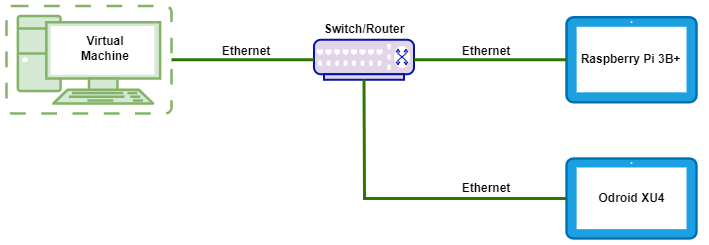
\includegraphics[width=1\textwidth]{images/Visual_representation_of_hardware_setup.png}
	\caption{Visual representation of the hardware setup}
	\label{fig:Visual_representation_of_hardware_setup}
\end{figure}
\par In order to implement the applications to visualise the usage of technologies several open source stacks such as scapy-someip \cite{scapy_someip}, the GENIVI vsomeip stack  \cite{b_genivi_vsomeip}, Rust based SOME/IP implementation \cite{rust_someip} were investigated. COVESA's (formerly known as GENIVI's) vsomeip stack appeared to be the most appropriate of the currently available implementations for this activity as it is based on POSIX and uses C++ programming language for the implementation. With the trend toward using Adaptive AUTOSAR\cite{b_adaptive_platform} in application software development, it makes sense to realize the concepts in a POSIX-based environment. 
 
\begin{figure}[!htb]
	\centering
		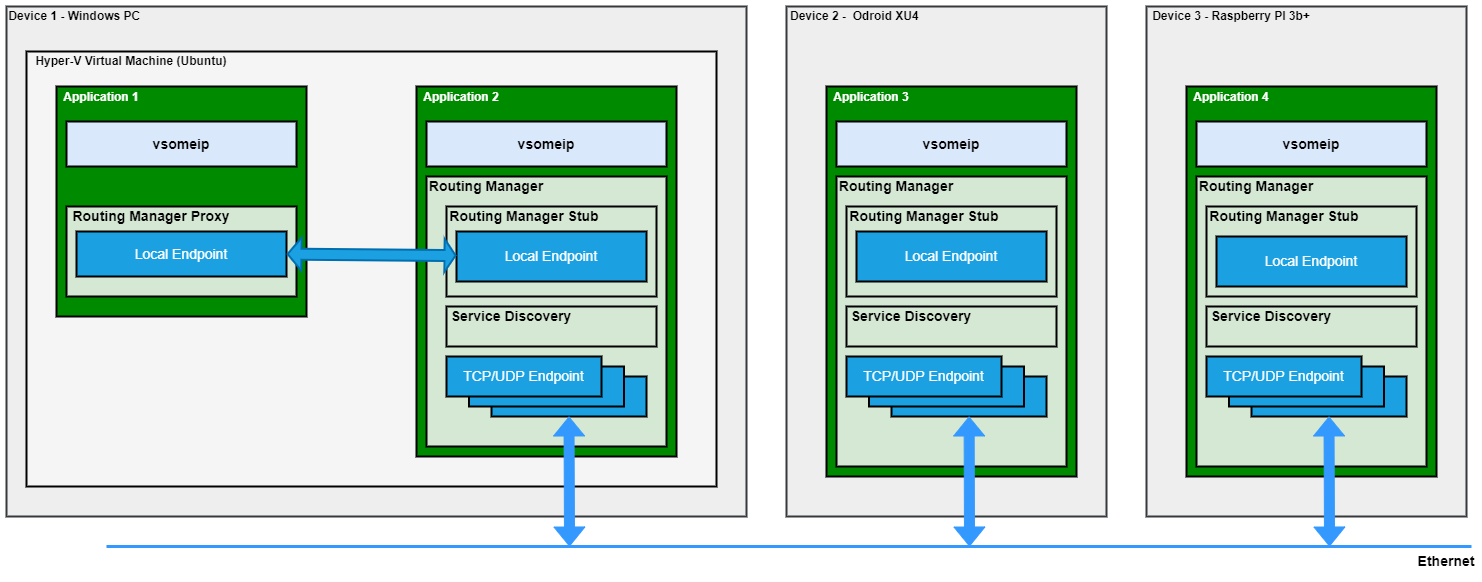
\includegraphics[width=1\textwidth]{images/SOMEIP_concept.png}
	\caption{SOME/IP concept}
	\label{fig:SOMEIP_concept}
\end{figure}




\section{Environment}
\subsection{Operating system}
Linux OS

\section{Target Hardware}
\subsection{Virtual Machine}
\subsection{Raspiberry Pi 3b+}
\subsection{Odroid XU4}

\section{Software}
\subsection{Target Libraries}
\subsubsection{GENIVI vsomeip stack}

\subsubsection{Other dependencies}
Boost

\subsection{Tools}
\subsubsection{Qt Creator}
Describe in brief about Qt Creator
\subsubsection{CMake}
Describe in brief about CMake
\subsubsection{PuTTY}
PuTTY is an SSH and telnet client, developed originally by Simon Tatham for the Windows platform\cite{b_putty}. PuTTY is open source software that is available with source code and is developed and supported by a group of volunteers\cite{b_putty}. This tool is required to run the terminals for Raspberry Pi3b+ and Odroid XU4 remotely on the host machine. This enables to smoothly switch between the target devices when running the applications on the target hardware respectively.

\section{Cross-compilation}
Every development board is embedded with a specific amount of RAM, storage capacity, input and output peripherals and other hardware components. Hosting the target environment on multiple boards can be complicated and time consuming. Furthermore, building target libraries on these boards can take a long time and may fail in some cases. To address these issues, it is worthwhile to setup a generic build environment on a single platform and build the projects for different targets accordingly. This process is called as cross-compilation. In this section, the process to setup a cross-compilation environment on the Linux platform is illustrated and along with it, the procedure to cross-compile boost libraries for Raspberry Pi and Odroid XU4 target platforms is demonstrated respectively.

\subsection{Installing cross compilers on the host machine}
In this section, the basic requirements to setup a cross-compilation tool-chain is described. Also, based on the requirements for the demonstration of the SOME/IP technology, build process for libraries such as Boost, CommonAPI, vsomeip and other relevant libraries are described in detail. 
\par In order to cross-compile, appropriate tool-chain packages has to be first setup in the host environment. The commands from the following listings are required to be run in a terminal window in the Linux machine. Please note that an active internet connection is required to download the packages from the server. 

\begin{lstlisting}[language=bash, caption={Command to install packages for ARM 32-bit (armv7) tool-chain}]
  user@machine:~$ sudo apt-get install gcc-arm-linux-gnueabihf
	g++-arm-linux-gnueabihf
\end{lstlisting}

\begin{lstlisting}[language=bash, caption={Command to install packages for ARM 64-bit(armv8) tool-chain}]
  user@machine:~$ sudo apt-get install gcc-aarch64-linux-gnu
	g++-aarch64-linux-gnu
\end{lstlisting}

\begin{lstlisting}[language=bash, caption={Command to install other required packages}]
  user@machine:~$ sudo apt-get install build-essential
	manpages-dev openjdk-8-jdk libssl-dev wireshark 
	g++-aarch64-linux-gnu
\end{lstlisting} 

\subsubsection{Installing Boost libraries}


\section{Demo Application}
\subsection{Server Application}
\subsection{Client Application}
\subsection{Comunication establishment between devices}
Configuration
